%% ---------------------------------------------------------------------------
%% intro.tex
%%
%% Introduction
%%
%% $Id: intro.tex 1477 2010-07-28 21:34:43Z palvarado $
%% ---------------------------------------------------------------------------

\chapter{Introduction}
\label{chp:intro}

\section{Video artifacts in live video streaming}
\label{sec:intro_artifacts}

Modern streaming services are fundamental instruments in today's industries, institutions, and every day life. Live video conferencing and streaming services became the principal mediums of communication for a large sector of national and global society during the recent COVID-19 pandemic, thus exemplifying the crucial role that these services now have. Current advances in network speed and digital technology have enabled these services to become commonplace in professional, academic, and recreational contexts. Therefore, there has been increased interest in ensuring a high quality of experience (QoE) for these services.

One of the main issues affecting the QoE of video conferencing and live streaming services are video artifacts, as mentioned in \cite{Vranjes2018, Korhonen2018}. In \cite{Greengrass2009}, video artifacts, or simply artifacts, are defined as distortions in the images displayed to the user with respect to the original captured images. According to \cite{Vranjes2018}, artifacts are primarily caused by errors or loss of data in the transmission of the video over the network, or by losses caused during video compression.

Figure \ref{fig:lossy_system} illustrates the basic structure of a lossy video system. In order to send video through a network, the video gets encoded into network packets, then sent through a transmission channel where the losses occur, then decoded into video with artifacts. Figure \ref{fig:frame_comparison} compares two versions of the same image. Figure \ref{fig:frame_comparison.a} contains no video artifacts and Figure \ref{fig:frame_comparison.b} contains video artifacts due to packet loss.

\begin{figure} [!h]
  \centering
  
  \includegraphics{lossy_system}
  
  \caption{Lossy video transmission system}
  \label{fig:lossy_system}

\end{figure}

\begin{figure} [!h]
  \centering
  
  \begin{subfigure}[t]{0.49\textwidth}
    \centering
    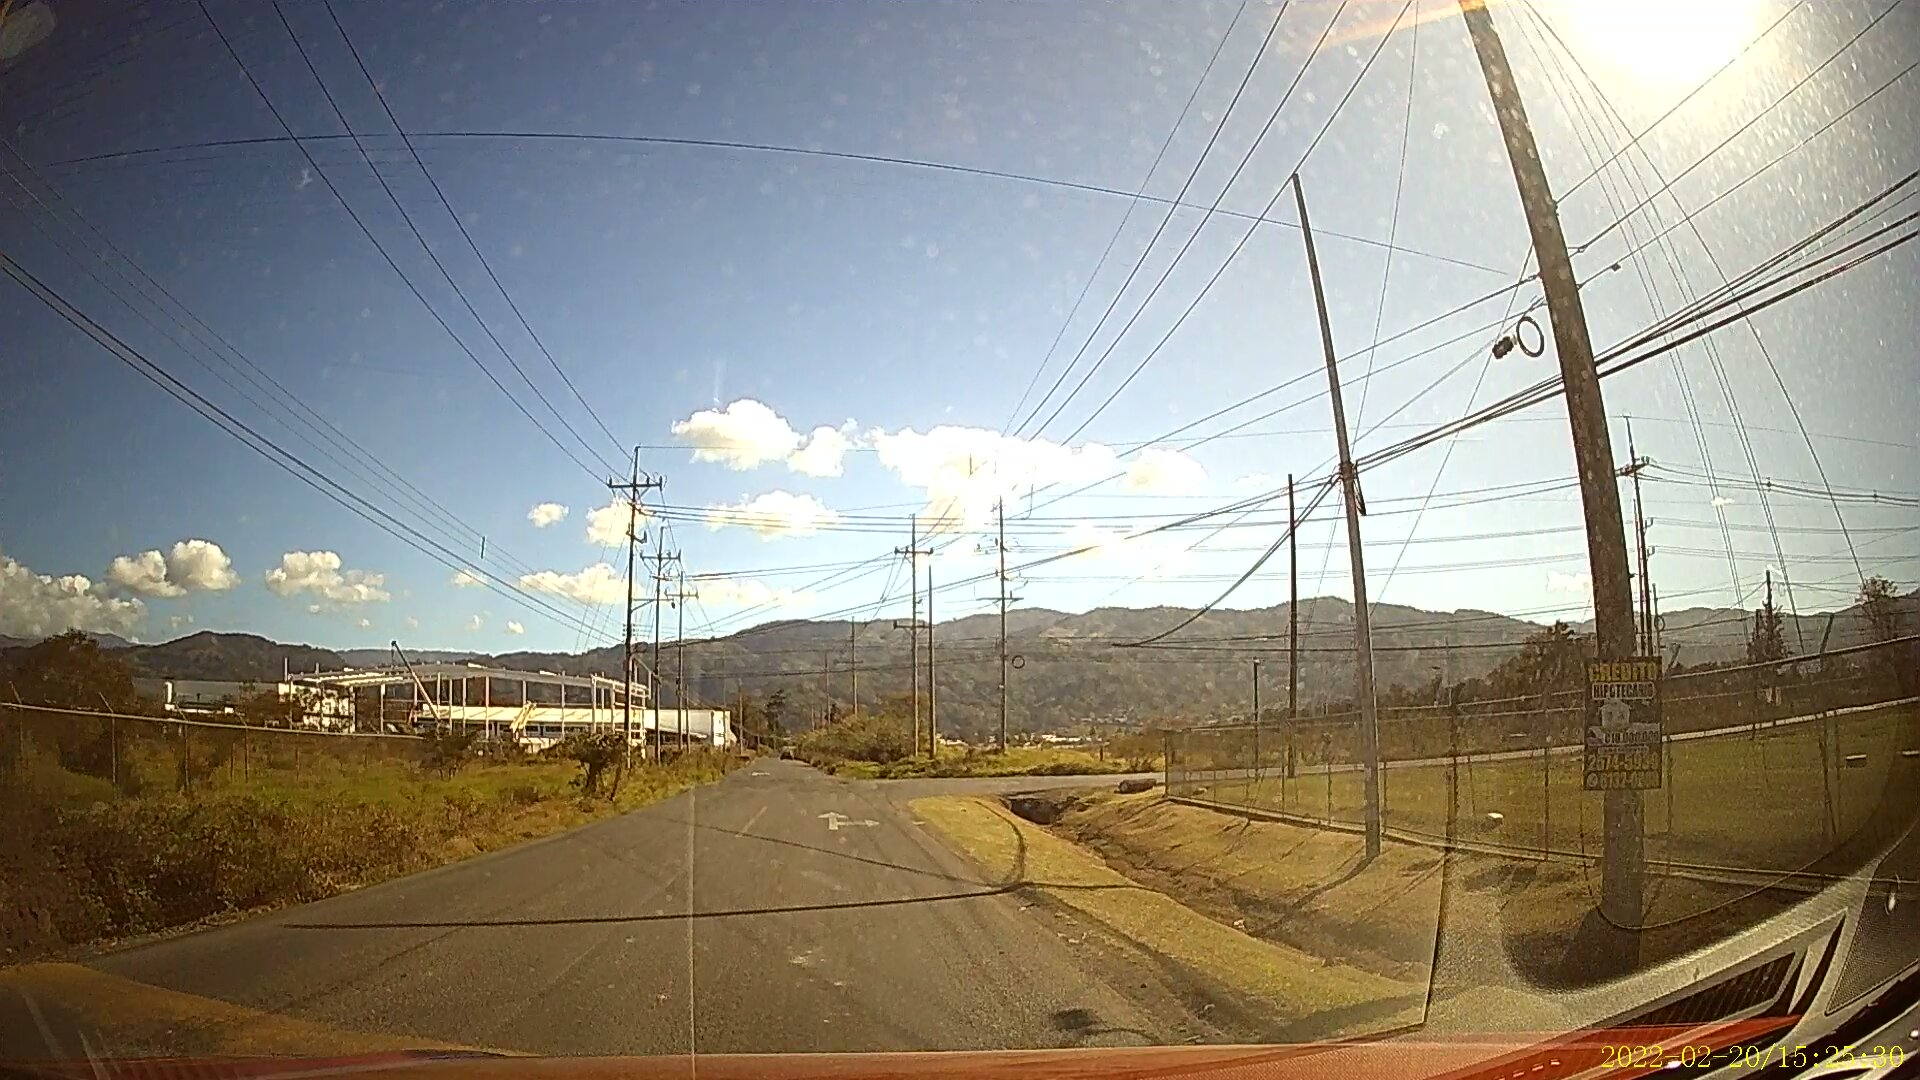
\includegraphics[width=\textwidth]{imgs_27}
    \caption{Frame with no video artifacts}
    \label{fig:frame_comparison.a}
  \end{subfigure}
  \hfill
  \begin{subfigure}[t]{0.49\textwidth}
    \centering
    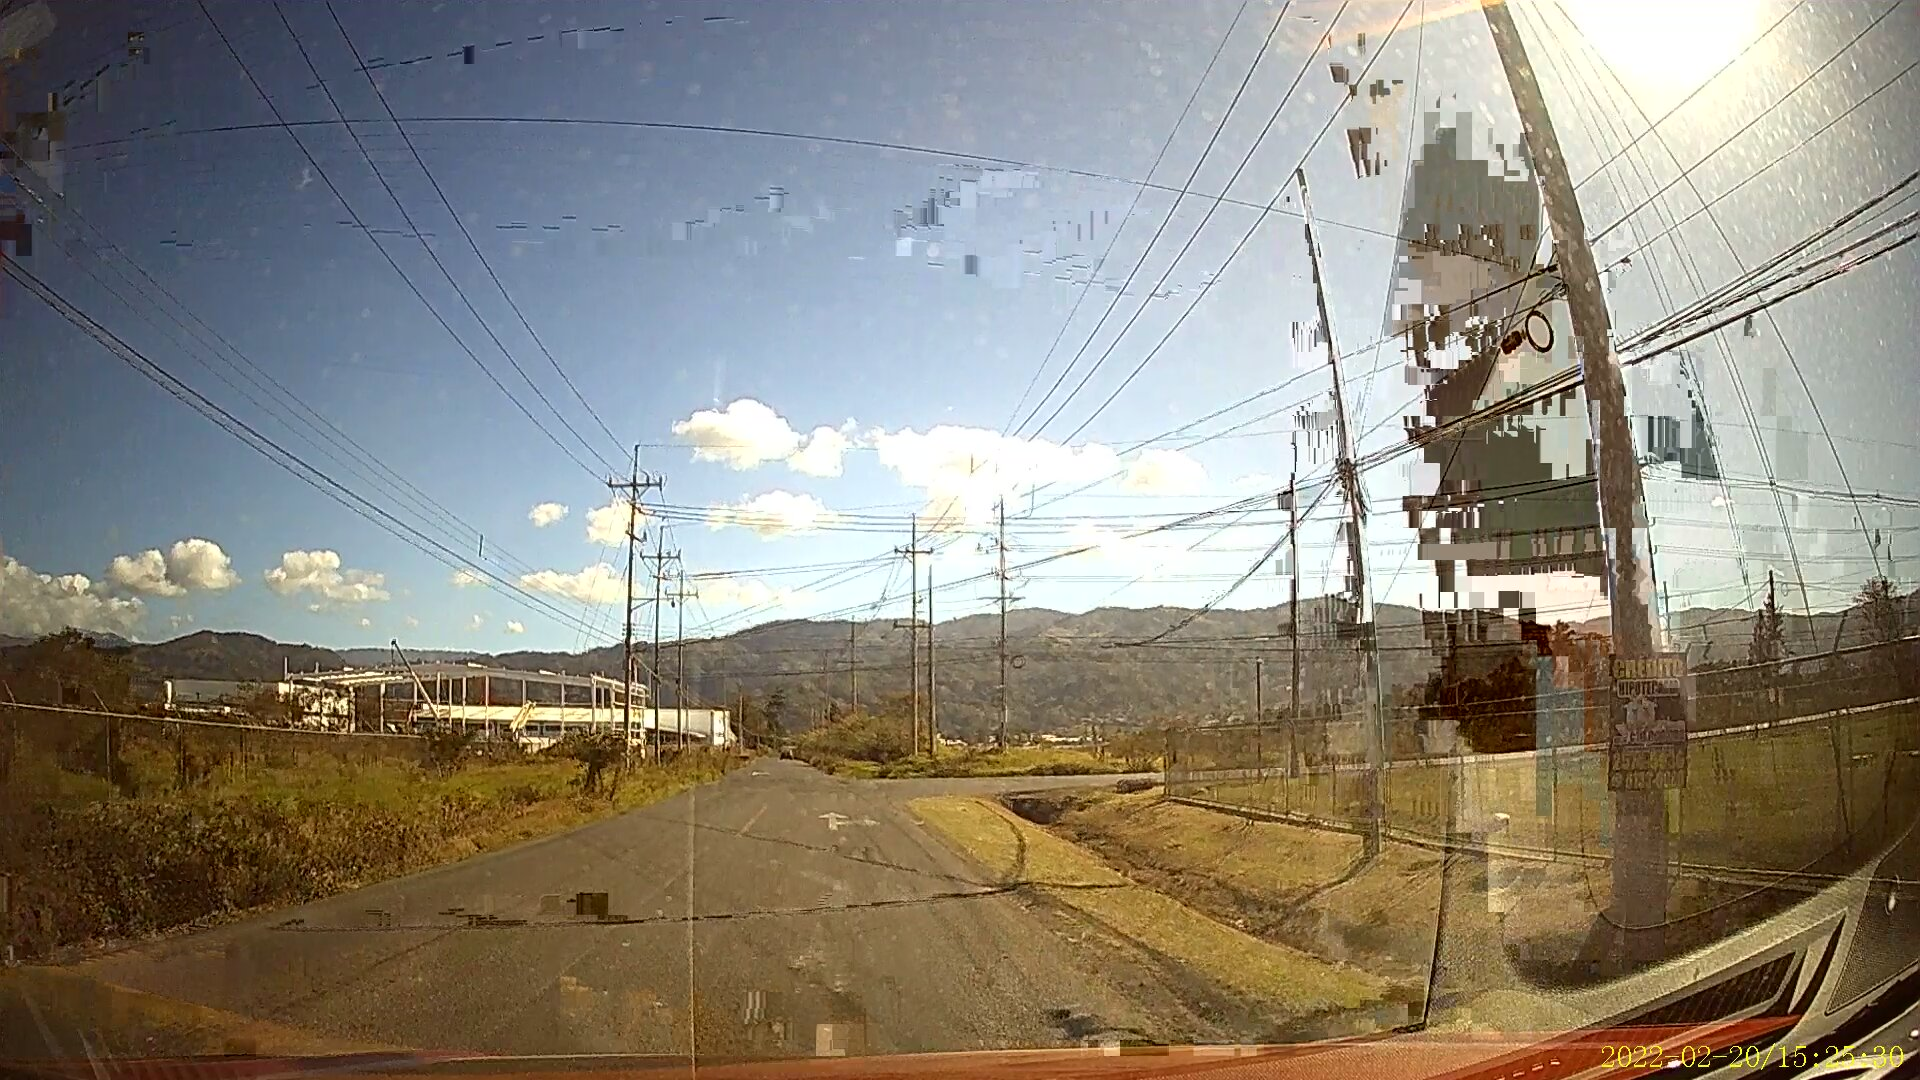
\includegraphics[width=\textwidth]{imgs_with_loss_27}
    \caption{Frame with video artifacts due to packet loss}
    \label{fig:frame_comparison.b}
  \end{subfigure}
  
  \caption{Comparison between a video frame with no artifacts and a video frame with artifacts caused by random h264 packet loss.}
  \label{fig:frame_comparison}

\end{figure}

There are methods to correct transmission errors in the transport layer or even in the video syntax layer, as mentioned in \cite{Sanyal2021}. In these cases, information is available on how the video packets are encoded, which simplifies the task of error detection and correction. When the user only has the decoded and decompressed information, it is necessary to use methods for artifact detection and correction that only have the raw video information, such as those of \cite{Vranjes2018, Sanyal2021,Goodall2019}. These methods are referred to as ``no-reference methods''.

Video artifacts result in loss of information from the original video. In video conferencing and live streaming applications, it is not possible to recover the lost data without affecting the user's QoE. In order to correct video artifacts, no-reference methods must infer the lost data. The process of restoring unknown areas of an image is called ``video inpainting'' \cite{Li2022, Zhou2021}. Video inpainting, or simply inpainting, is commonly used to remove the presence of objects in a video or image, but can be used to reconstruct areas of an image affected by video artifacts, as is done in \cite{Dong2023, Brenes2022}.

Modern inpainting algorithms use machine learning models. The inpainters of \cite{Li2022, Zhou2021, Liu2021} use ``transformers''. Transformers are machine learning models with outstanding results for signal restoration tasks, but they are slow and require signficant processing power. GPUs and other hardware accelerators are used in order to optimize the performance of these models.

Inpainting models such as \cite{Li2022} require binary masks to identify the areas to be reconstructed. For this reason, the location of video artifacts must be detected and binary masks must be generated and then used in the image restoration stage.

\cite{Greengrass2009, Glavota2016} classify the various types of artifacts generated by packet loss. These studies also describe the statistical properties of video artifacts. For example, certain video artifacts tend to have high-contrast vertical and horizontal edges that can be detected by high-pass filters. In the MPEG and H.26x video compression standards, the pixels of an image are grouped into ``macroblocks'', which are groups of $16 \times 16$ pixels in the image. Losses of packets containing macroblock information result in artifacts with well-defined edges \cite{Vranjes2019, Glavota2018}.

The artifact detection methods from \cite{Vranjes2018, Glavota2018} focus on filtering algorithms that do not involve machine learning. These methods can process standard definition video at 30 frames per second without GPU acceleration, but they oversimplify the characteristics of video artifacts and fail to perform well on the artifact detection task. The detectors of \cite{Goodall2019, Rajasekar2020} use neural network classifiers. These methods generalize better than filtering algorithms, but they require GPU accelerators in order to achieve comparable framerates with the filtering algorithms.

\section{The dispTEC2-2022 project}
\label{sec:intro_disptec}

During 2022, RidgeRun LLC and SIPLab developed the dispTEC2-2022 (Disptec) project with the objective of building a Video Restoration System using DeepLearning. The project was developed on the Nvidia Jetson TX2 Embedded System. This machine has a 256 CUDA-core GPU, a Quad-core ARM CPU and a Dual-core Denver CPU. Disptec found no activation method for the Denver CPU and the Jetson TX2 machine was effectively a 4-core machine.

The resulting system was composed of an Artifact Detection System and an Inpainter System \cite{Brenes2022}. The system was capable of processing a video frame by frame. For each frame it could simulate randomly linear H264 packet losses, generate a binary detection mask based on the ground truth artifact measure, and then feed it along with the lossy frame into an inpainter transformer to produce a restored frame. \cite{Brenes2022} optimized the Inpainter System through a series of arquitectural redesigns. He finally concluded that the system could reach a framerate from 0.8 to 1.67 frames per second on the Nvidia Jetson TX2, optimizing the Inpainter's Torch backend for the GPU with CUDA.

However, this system cannot be used in practice because it relies on knowing the original frames in order to generate the binary detection masks. The system requires an artifact detector that can generate the masks from the lossy frames alone.

\section{The Artifact Detector Problem}
\label{sec:intro_problem}

The dispTEC2-2022 Video Restoration System concluded without a proper artifact detector. Part of dispTEC2-2022 entailed the search and development of an apropiate artifact detector for the system. The artifact detector was expected to run on the ARM 4-core CPU alone, in order not to interfere with the CUDA-accelerated inpainting model and possibly decrease the inpainting speed. As a first approach, the dispTEC2-2022 team implemented the Packet Loss Detection Algorithm (PLDA) from \cite{Vranjes2018}. When testing the algorithm inside a gstreamer element, the algorithm could process a 720p video at $23,0$ frames per second.  After extensive testing of the algorithm using the Non-dominated Sorting Genetic Algorithm (NSGA-II), the dispTEC2-2022 team found no suitable parameters that allowed the detector to perform well on the detection task.

The dispTEC2-2022 team also developed a second artifact detection approach based on Random Decision Forests (RDF) \cite{Breiman2001}. In this approach, the RDF classifiers operated directly on each raw video frame and could achieve slightly better detection results than a random classifier. This classifier was trained on 200 frames from a training dataset containing only 2 video content types. When testing the RDF approach inside a gstreamer element, the algorithm could process 720p video at $26,6$ frames per second.

These results suggested that the RDF classifers were capable of learning artifact detection from the raw frame information. These results also suggested that the algorithm could be optimized to reach a framerate of $30$ frames per second.

\todo{Find PLDA framerate and metrics}
\todo{Find RDF framerate and metrics}

\section{Rangerx}
\label{sec:intro_detector}

The dispTEC2-2022 Video Restoration System is designed to restore video with artifacts frame by frame. Figure \ref{fig:restoration_system_overview} describes the general structure of the system. The figure shows a small section of an input frame with artifacts and the expected output from the system.

\begin{figure} [!h]
  \centering
  
  \includegraphics{video_inpainter_general}
  
  \caption{Video restoration system overview.}
  \label{fig:restoration_system_overview}

\end{figure}

The system has two main components: the Artifact Detection System and the Inpainting System. Figure \ref{fig:restoration_system_steps} displays the inner structure of the Video Restoration System. The Artifact Detection System takes the frames with artifacts and generates binary detection masks. The Inpainting System takes the frames with artifacts and the detection masks. It then generates the restored video frames.

\begin{figure} [!h]
  \centering
  
  \includegraphics{video_inpainter_steps}
  
  \caption{Video restoration process. }
  \label{fig:restoration_system_steps}

\end{figure}

This project proposes Rangerx, a new Artifact Detection System. Rangerx aims to improve over the dispTEC2-2022 detection system by expanding the training dataset, redesigning and optimizing the feature extraction strategy, and replacing the RDF backend with the optimized Ranger C++ Core Library.

Random Decision Forests are subject to overfitting when training with small, highly self correlated datasets \cite{Breiman2001}. Rangerx expands the dataset with diverse video content in order to reduce the RDF detector overfitting.

The dispTEC2-2022 research found that RDF detectors could learn from raw image data. However, the feature extraction strategy can be improved by considering some of the statistical properties of artifacts described in \cite{Vranjes2019, Glavota2018}. Rangerx filters the raw image data to detect high contrast vertical and horizontal borders, then generates 132 statistical features from the filtered results.

Random Decision Forests agregate the results of a set of independent Decision Tree Classifiers. The dispTEC2-2022 RDF library ran the individual classifers consecutivelly. In contrast, the Ranger C++ Core Library runs the individual classifiers concurrently in seperate threads. Rangerx replaces the dispTEC2-2022 RDF backend with Ranger in order to improve the detection speed.

\section{Project objectives and document structure}
\label{sec:intro_objectives}

The aim of this project is to develop Rangerx, a real-time Artifact Detection System that can generate binary detection masks from video with artifacts. This system should improve over the dispTEC2-2022 system. This project focuses on video artifacts produced by decoding H264 packet loss. The system should run on an NVIDIA Jetson TX2 without using the GPU, which should be verified with CPU and GPU profiles. The training dataset should be expanded from the original 200 frames and 2 video content types to at least 18 video content types with 200 frames each. The new Artifact Detection System should achieve at least 70\% in both precision and recall detection metrics. The new system should provide a testing tool to verify these metrics. The new system should achieve a framerate of 30 frames per second. The new system should also provide a testing tool to verify the framerate.

The first milestone in the development of Rangerx is the expansion of the training dataset. This not only requires obtaining new video, but also requires procesing the videos to generate the ground truth binary masks that will be used as labels in the training procedure. \cite{Brenes2022} provides a similar tool, which can be used as a starting point. The final dataset should contain 18 video content types with at least 3 different illumination types.

The second milestone in the development of Rangerx is implementing the training procedure, the feature selection and the replacement of the RDF backend. These changes are aimed at improving the precision and recall detection metrics up to 70\%. Rangerx should provide a tool that can verify the detection performance against a test dataset.

The third milestone in the development of Rangerx is optimizing the feature selection and detection procedures in order to achieve real-time performance. Rangerx should provide a tool that can verify a framerate of 30 frames per second while testing the system on an input video.

The following chapters explore the project's main theoretical aspects, a detailed description of Rangerx and the final results. Chapter \ref{ch:marco} explores several theoretical concepts used in the development of Rangerx. Chapter \ref{ch:solucion} describes Rangerx in detail. Chapter \ref{chp:results} discusses Rangerx's final results. Chapter \ref{chp:conclusions} summarizes the project's main accomplishments, as well as future work related to Rangerx and dispTEC2-2022's Video Restoration System.
